% This file is generated by the MATLAB m-file laprint.m. It can be included
% into LaTeX documents using the packages graphicx, color and psfrag.
% It is accompanied by a postscript file. A sample LaTeX file is:
%    \documentclass{article}\usepackage{graphicx,color,psfrag}
%    \begin{document}% This file is generated by the MATLAB m-file laprint.m. It can be included
% into LaTeX documents using the packages graphicx, color and psfrag.
% It is accompanied by a postscript file. A sample LaTeX file is:
%    \documentclass{article}\usepackage{graphicx,color,psfrag}
%    \begin{document}% This file is generated by the MATLAB m-file laprint.m. It can be included
% into LaTeX documents using the packages graphicx, color and psfrag.
% It is accompanied by a postscript file. A sample LaTeX file is:
%    \documentclass{article}\usepackage{graphicx,color,psfrag}
%    \begin{document}% This file is generated by the MATLAB m-file laprint.m. It can be included
% into LaTeX documents using the packages graphicx, color and psfrag.
% It is accompanied by a postscript file. A sample LaTeX file is:
%    \documentclass{article}\usepackage{graphicx,color,psfrag}
%    \begin{document}\input{bdry}\end{document}
% See http://www.mathworks.de/matlabcentral/fileexchange/loadFile.do?objectId=4638
% for recent versions of laprint.m.
%
% created by:           LaPrint version 3.16 (13.9.2004)
% created on:           20-Feb-2012 17:38:36
% eps bounding box:     15 cm x 11.2299 cm
% comment:              
%
\begin{psfrags}%
\psfragscanon%
%
% text strings:
\psfrag{s10}[][]{\color[rgb]{0,0,0}\setlength{\tabcolsep}{0pt}\begin{tabular}{c} \end{tabular}}%
\psfrag{s11}[][]{\color[rgb]{0,0,0}\setlength{\tabcolsep}{0pt}\begin{tabular}{c} \end{tabular}}%
\psfrag{s12}[l][l]{\color[rgb]{0,0,0}quasi-bicubic}%
\psfrag{s13}[l][l]{\color[rgb]{0,0,0}truth}%
\psfrag{s14}[l][l]{\color[rgb]{0,0,0}bilinear}%
\psfrag{s15}[l][l]{\color[rgb]{0,0,0}bicubic}%
\psfrag{s16}[l][l]{\color[rgb]{0,0,0}Collatz-Keys}%
\psfrag{s17}[l][l]{\color[rgb]{0,0,0}quasi-bicubic}%
%
% xticklabels:
\psfrag{x01}[t][t]{0}%
\psfrag{x02}[t][t]{}%
\psfrag{x03}[t][t]{0.01}%
\psfrag{x04}[t][t]{}%
\psfrag{x05}[t][t]{0.02}%
\psfrag{x06}[t][t]{}%
\psfrag{x07}[t][t]{0.03}%
\psfrag{x08}[t][t]{}%
\psfrag{x09}[t][t]{0.04}%
%
% yticklabels:
\psfrag{v01}[r][r]{0}%
\psfrag{v02}[r][r]{0.2}%
\psfrag{v03}[r][r]{0.4}%
\psfrag{v04}[r][r]{0.6}%
\psfrag{v05}[r][r]{0.8}%
\psfrag{v06}[r][r]{1}%
%
% Figure:
\resizebox{0.5\columnwidth}{!}{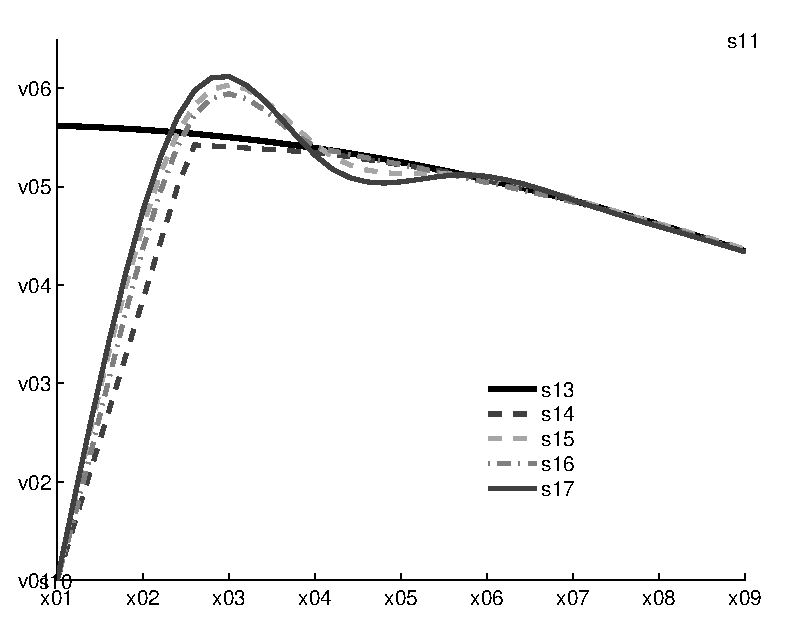
\includegraphics{figures/bdry.eps}}%
\end{psfrags}%
%
% End bdry.tex
\end{document}
% See http://www.mathworks.de/matlabcentral/fileexchange/loadFile.do?objectId=4638
% for recent versions of laprint.m.
%
% created by:           LaPrint version 3.16 (13.9.2004)
% created on:           20-Feb-2012 17:38:36
% eps bounding box:     15 cm x 11.2299 cm
% comment:              
%
\begin{psfrags}%
\psfragscanon%
%
% text strings:
\psfrag{s10}[][]{\color[rgb]{0,0,0}\setlength{\tabcolsep}{0pt}\begin{tabular}{c} \end{tabular}}%
\psfrag{s11}[][]{\color[rgb]{0,0,0}\setlength{\tabcolsep}{0pt}\begin{tabular}{c} \end{tabular}}%
\psfrag{s12}[l][l]{\color[rgb]{0,0,0}quasi-bicubic}%
\psfrag{s13}[l][l]{\color[rgb]{0,0,0}truth}%
\psfrag{s14}[l][l]{\color[rgb]{0,0,0}bilinear}%
\psfrag{s15}[l][l]{\color[rgb]{0,0,0}bicubic}%
\psfrag{s16}[l][l]{\color[rgb]{0,0,0}Collatz-Keys}%
\psfrag{s17}[l][l]{\color[rgb]{0,0,0}quasi-bicubic}%
%
% xticklabels:
\psfrag{x01}[t][t]{0}%
\psfrag{x02}[t][t]{}%
\psfrag{x03}[t][t]{0.01}%
\psfrag{x04}[t][t]{}%
\psfrag{x05}[t][t]{0.02}%
\psfrag{x06}[t][t]{}%
\psfrag{x07}[t][t]{0.03}%
\psfrag{x08}[t][t]{}%
\psfrag{x09}[t][t]{0.04}%
%
% yticklabels:
\psfrag{v01}[r][r]{0}%
\psfrag{v02}[r][r]{0.2}%
\psfrag{v03}[r][r]{0.4}%
\psfrag{v04}[r][r]{0.6}%
\psfrag{v05}[r][r]{0.8}%
\psfrag{v06}[r][r]{1}%
%
% Figure:
\resizebox{0.5\columnwidth}{!}{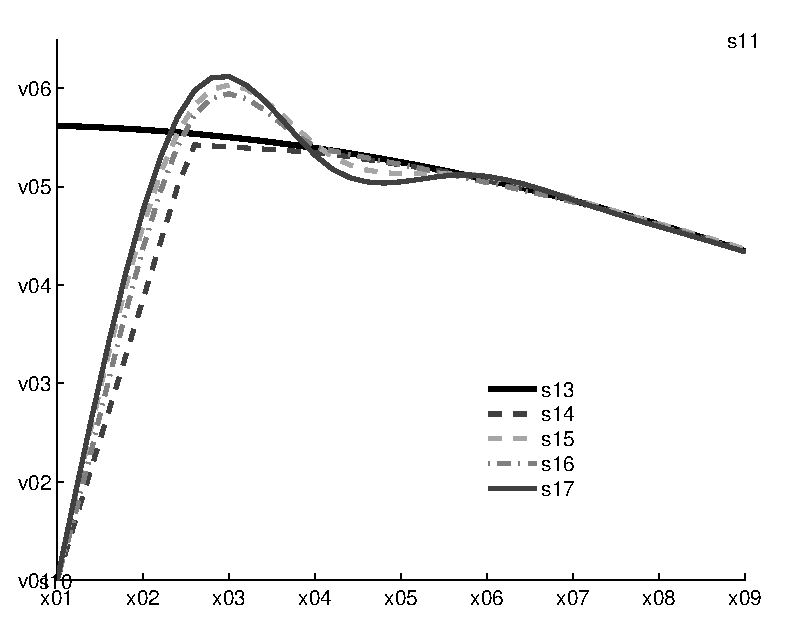
\includegraphics{figures/bdry.eps}}%
\end{psfrags}%
%
% End bdry.tex
\end{document}
% See http://www.mathworks.de/matlabcentral/fileexchange/loadFile.do?objectId=4638
% for recent versions of laprint.m.
%
% created by:           LaPrint version 3.16 (13.9.2004)
% created on:           20-Feb-2012 17:38:36
% eps bounding box:     15 cm x 11.2299 cm
% comment:              
%
\begin{psfrags}%
\psfragscanon%
%
% text strings:
\psfrag{s10}[][]{\color[rgb]{0,0,0}\setlength{\tabcolsep}{0pt}\begin{tabular}{c} \end{tabular}}%
\psfrag{s11}[][]{\color[rgb]{0,0,0}\setlength{\tabcolsep}{0pt}\begin{tabular}{c} \end{tabular}}%
\psfrag{s12}[l][l]{\color[rgb]{0,0,0}quasi-bicubic}%
\psfrag{s13}[l][l]{\color[rgb]{0,0,0}truth}%
\psfrag{s14}[l][l]{\color[rgb]{0,0,0}bilinear}%
\psfrag{s15}[l][l]{\color[rgb]{0,0,0}bicubic}%
\psfrag{s16}[l][l]{\color[rgb]{0,0,0}Collatz-Keys}%
\psfrag{s17}[l][l]{\color[rgb]{0,0,0}quasi-bicubic}%
%
% xticklabels:
\psfrag{x01}[t][t]{0}%
\psfrag{x02}[t][t]{}%
\psfrag{x03}[t][t]{0.01}%
\psfrag{x04}[t][t]{}%
\psfrag{x05}[t][t]{0.02}%
\psfrag{x06}[t][t]{}%
\psfrag{x07}[t][t]{0.03}%
\psfrag{x08}[t][t]{}%
\psfrag{x09}[t][t]{0.04}%
%
% yticklabels:
\psfrag{v01}[r][r]{0}%
\psfrag{v02}[r][r]{0.2}%
\psfrag{v03}[r][r]{0.4}%
\psfrag{v04}[r][r]{0.6}%
\psfrag{v05}[r][r]{0.8}%
\psfrag{v06}[r][r]{1}%
%
% Figure:
\resizebox{0.5\columnwidth}{!}{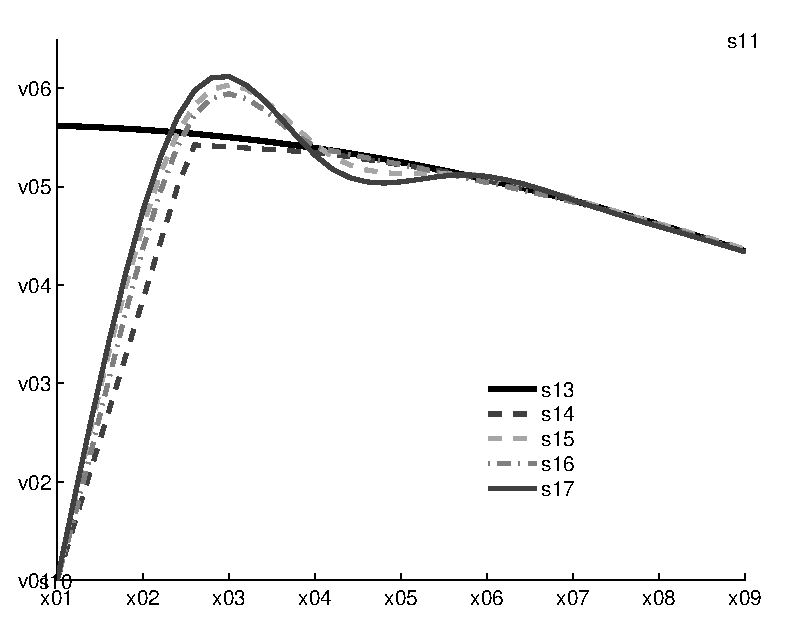
\includegraphics{figures/bdry.eps}}%
\end{psfrags}%
%
% End bdry.tex
\end{document}
% See http://www.mathworks.de/matlabcentral/fileexchange/loadFile.do?objectId=4638
% for recent versions of laprint.m.
%
% created by:           LaPrint version 3.16 (13.9.2004)
% created on:           20-Feb-2012 17:38:36
% eps bounding box:     15 cm x 11.2299 cm
% comment:              
%
\begin{psfrags}%
\psfragscanon%
%
% text strings:
\psfrag{s10}[][]{\color[rgb]{0,0,0}\setlength{\tabcolsep}{0pt}\begin{tabular}{c} \end{tabular}}%
\psfrag{s11}[][]{\color[rgb]{0,0,0}\setlength{\tabcolsep}{0pt}\begin{tabular}{c} \end{tabular}}%
\psfrag{s12}[l][l]{\color[rgb]{0,0,0}quasi-bicubic}%
\psfrag{s13}[l][l]{\color[rgb]{0,0,0}truth}%
\psfrag{s14}[l][l]{\color[rgb]{0,0,0}bilinear}%
\psfrag{s15}[l][l]{\color[rgb]{0,0,0}bicubic}%
\psfrag{s16}[l][l]{\color[rgb]{0,0,0}Collatz-Keys}%
\psfrag{s17}[l][l]{\color[rgb]{0,0,0}quasi-bicubic}%
%
% xticklabels:
\psfrag{x01}[t][t]{0}%
\psfrag{x02}[t][t]{}%
\psfrag{x03}[t][t]{0.01}%
\psfrag{x04}[t][t]{}%
\psfrag{x05}[t][t]{0.02}%
\psfrag{x06}[t][t]{}%
\psfrag{x07}[t][t]{0.03}%
\psfrag{x08}[t][t]{}%
\psfrag{x09}[t][t]{0.04}%
%
% yticklabels:
\psfrag{v01}[r][r]{0}%
\psfrag{v02}[r][r]{0.2}%
\psfrag{v03}[r][r]{0.4}%
\psfrag{v04}[r][r]{0.6}%
\psfrag{v05}[r][r]{0.8}%
\psfrag{v06}[r][r]{1}%
%
% Figure:
\resizebox{0.5\columnwidth}{!}{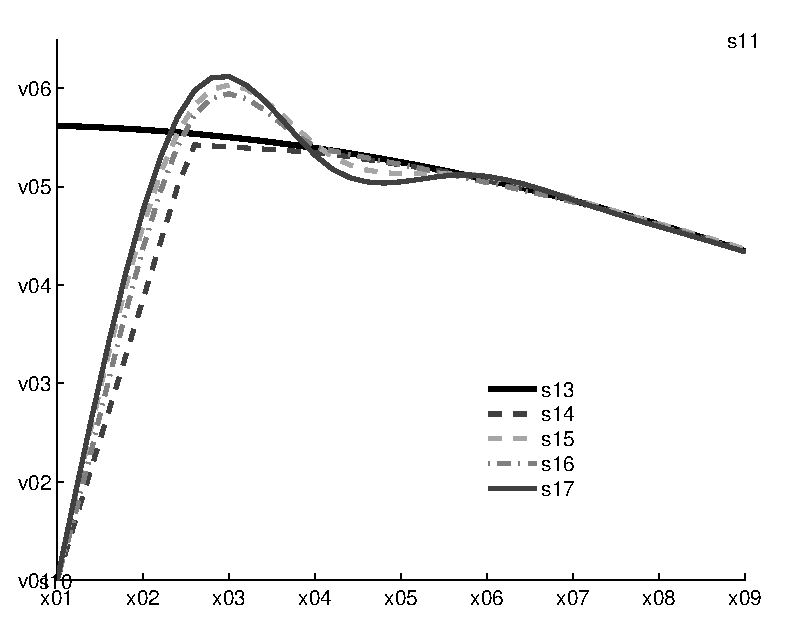
\includegraphics{figures/bdry.eps}}%
\end{psfrags}%
%
% End bdry.tex
